\documentclass[english,11pt,a4paper,titlepage]{report}
\usepackage[T1]{fontenc}
\usepackage{graphicx}
\usepackage{amsmath}
\usepackage{babel}
\usepackage{listings}
\usepackage{microtype}
\title{Handin 3 - Semi-supervised deep learning}
\author{Rasmus Freund - 201700273}
\lstset{numbers=left,language=Python,frame=single,showtabs=false,breaklines=true,tabsize=4,xrightmargin=-20mm}
\begin{document}
	\maketitle
	\subsection*{Short answer questions}	
	\begin{itemize}
		\item Where are we ensuring that the finetuning does not affect the feature extractor?
		\begin{itemize}
			\item The \verb*|Net| class has been created with separate components for feature extraction and classification; which has additionally been split into two layers: \verb*|pretrainer| and \verb*|generalizer|. When finetuning (\verb*|optim.SGD(network.generalizer.parameters(),lr=0.01)|) we only update the \verb*|generalizer| parameters, not those of the feature extractor.  
		\end{itemize}
		\item How dose the code work that gets $s$ samples per class for the pre-training dataset
		\begin{itemize}
			\item The \verb*|get_subsampled_dataset| function iterates over each class in the dataset. For each class, it finds the indices where the target label matches the current class and randomly selects $k$ indices from that list which are then appended to the subset.
		\end{itemize}
		\item What is the \verb*|forward_call| parameter responsible for in the \verb*|train()| method (located in \verb*|network_training.py|)?
		\begin{itemize}
			\item It performs a forward pass through the network, calculating the loss.
		\end{itemize}
		\item Describe how the \verb*|augment()| method works (located \verb*|augmentations.py|).
		\begin{itemize}
			\item The function iterates through the batch of images, randomly selects another image from the batch \\(\verb*|merge_indices[i]=np.random.choice(...)|). The current image (i) is excluded from the pool, so we're never getting an augment where an image has been augmented with itself. Augmentation is then applied (either mixup or collage), resulting in a new image and an interpolation value.
		\end{itemize}
		\item If we pre-train and finetune on the same dataset, is there any reason to do the finetuning step?
		\begin{itemize}
			\item Typically, no. However, there might be specific cases where this could be beneficial. One example could be transfer learning where we could pre-train the model as a simple classification network. After that, the fine-tuning head could then be utilized for more specific tasks.
		\end{itemize}
	\end{itemize}
	\subsection*{Predictions}
	\begin{itemize}
		\item Will the collage and mixup data augmentations help achieve higher finetune accuracies? Which do you expect will be more effective?
		\begin{itemize}
			\item I doubt that data augmentation is going to improve accuracy in the case of these data sets. Changing the information in the images through augmentation is also going to change the true "meaning" of those images, since we're dealing with numbers and letters. Of the two types of augmentation, I suspect that mixup might perform better, since the entire structure of each number/letter will be kept in the augmented data.
		\end{itemize}
		\item What relationship do you expect between the number of samples in the pre-training dataset and the finetuning accuracy? Does this change with data augmentations?
		\begin{itemize}
			\item Generally, more samples in the pre-training should improve the accuracy of the fine-tuning head. However, given that the data is relatively simple and present clear patterns, a plateau is likely to be reached fairly quickly in terms of amount of training samples being used. Beyond this plateau, increasing the amount of samples will probably not lead to significant increases in accuracy. While data augmentation is, under most circumstances, a good way to increase accuracy when training on sparse data, I suspect it won't have a great impact in this network, mainly due to the reasons listed in the answer to the previous question.
		\end{itemize}
	\end{itemize}
	
	\newpage
	
	\subsection*{Discussion}
	\begin{figure}[h]
		\centering
		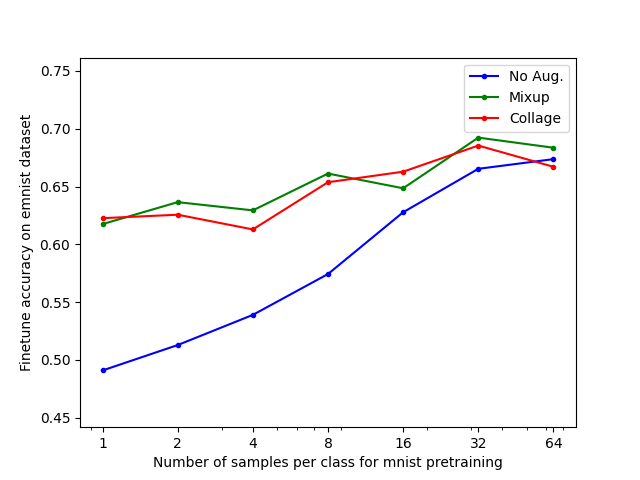
\includegraphics[width=0.7\linewidth]{semisupervised_deep_learning/Figure_1}
		\caption{Finetune accuracy of the network on the EMNIST dataset based on number of samples per class when pre-training on the MNIST dataset. Default settings for the network were used when creating this plot.}
		\label{fig:figure1}
	\end{figure}
	
	\begin{itemize}
		\item How does the number of samples per class affect training performance? Does this get affected by the augmentations?
		\begin{itemize}
			\item When applying no augmentation, increasing the amount of samples per class always increases accuracy of the model, as seen in \ref{fig:figure1}. However, the difference in accuracy between 32 and 64 samples is relatively minor, indicating that the model is unlikely to get much better with additional samples. Using augmentations improves the performance of the model, especially at low number of samples per class. At a single sample per class, the accuracy is increased from about 50\% to about 62\% for both types of augmentation. This difference decreases as the number of samples increases, to the point where there is little to no difference between the three options (no augmentation, collage, or mixup). The difference in accuracy based on number of samples is less dramatic on the models that are utilizing augmentation. At 1 sample per class both the mixup and collage models sit at about 62\% accuracy, whereas the maximum accuracy, reached at 32 samples per class, is approximately 68\%. The performance of augmentation models will be discussed in further detail below.\\
			\\
		\end{itemize}
		\item Which augmentation performs better? Why?
		\begin{itemize}
			\item 
		\end{itemize}
		\item Does finetuning and pre-training on the same dataset obtain better performance than pre-training on one dataset and finetuning on another? Why?
		\begin{itemize}
			\item 
		\end{itemize}
	\end{itemize}
	
	
\end{document}
